\documentclass[11pt]{article}
\usepackage[margin=12mm]{geometry}
\usepackage{newtxtext,newtxmath} % Times-like serif for publication style
\usepackage{tikz}
\usetikzlibrary{arrows.meta,positioning,calc}

\pagestyle{empty}

\begin{document}

% -------------------------------------------------------------------
% Figure 5.19 standalone source (pdflatex-ready)
% Tweak guide:
% 1) Vertical spacing: change node distance below.
% 2) Box widths: adjust text width in styles main/pivot/reject/final.
% 3) Font scale: change font=\small to \footnotesize or \normalsize.
% -------------------------------------------------------------------
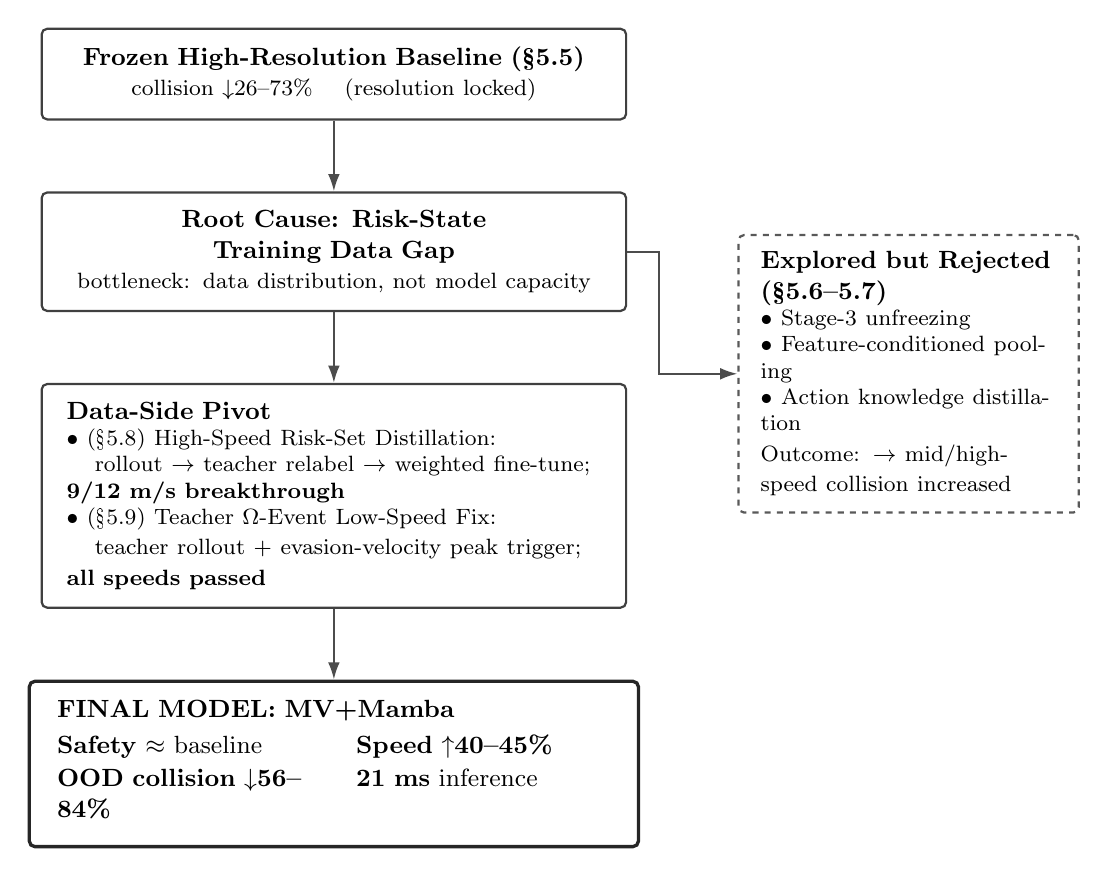
\begin{tikzpicture}[
    font=\small,
    node distance=9mm,
    main/.style={
        draw=black!75,
        line width=0.8pt,
        rounded corners=2pt,
        align=center,
        inner xsep=9pt,
        inner ysep=6.5pt,
        text width=0.56\linewidth
    },
    pivot/.style={
        draw=black!75,
        line width=0.8pt,
        rounded corners=2pt,
        align=left,
        inner xsep=9pt,
        inner ysep=6.5pt,
        text width=0.56\linewidth
    },
    reject/.style={
        draw=black!65,
        dash pattern=on 2.2pt off 2.2pt,
        line width=0.8pt,
        rounded corners=2pt,
        align=left,
        inner xsep=8pt,
        inner ysep=6pt,
        text width=0.31\linewidth
    },
    final/.style={
        draw=black!85,
        line width=1.2pt, % visual anchor emphasis
        rounded corners=2pt,
        align=left,
        inner xsep=10pt,
        inner ysep=7pt,
        text width=0.58\linewidth
    },
    arrow/.style={-{Latex[length=2.2mm,width=1.5mm]}, line width=0.8pt, draw=black!70}
]

% Left main pipeline (A -> B -> C -> D)
\node[main] (baseline) {
\textbf{Frozen High-Resolution Baseline (\S5.5)}\\
{\footnotesize collision $\downarrow$26--73\% \quad (resolution locked)}
};

\node[main, below=of baseline] (rootcause) {
\textbf{Root Cause: Risk-State Training Data Gap}\\
{\footnotesize bottleneck: data distribution, not model capacity}
};

\node[pivot, below=of rootcause] (pivot) {
\textbf{Data-Side Pivot}\\
{\footnotesize
$\bullet$ (\S5.8) High-Speed Risk-Set Distillation:\\
\hspace*{1.2em}rollout $\rightarrow$ teacher relabel $\rightarrow$ weighted fine-tune; \textbf{9/12 m/s breakthrough}\\
$\bullet$ (\S5.9) Teacher $\Omega$-Event Low-Speed Fix:\\
\hspace*{1.2em}teacher rollout + evasion-velocity peak trigger; \textbf{all speeds passed}
}
};

\node[final, below=of pivot] (finalmodel) {
\textbf{FINAL MODEL: MV+Mamba}\\[2pt]
\begingroup
\renewcommand{\arraystretch}{1.1}
\begin{tabular}{@{}p{0.48\linewidth}p{0.48\linewidth}@{}}
\textbf{Safety} $\approx$ baseline & \textbf{Speed} $\uparrow$\textbf{40--45\%}\\
\textbf{OOD collision} $\downarrow$\textbf{56--84\%} & \textbf{21 ms} inference
\end{tabular}
\endgroup
};

\draw[arrow] (baseline) -- (rootcause);
\draw[arrow] (rootcause) -- (pivot);
\draw[arrow] (pivot) -- (finalmodel);

% Right consolidated rejection panel
\coordinate (ranchor) at ($(rootcause.east)!0.5!(pivot.east)$);
\node[reject, anchor=west] (rejected) at ($(ranchor)+(14mm,0)$) {
\textbf{Explored but Rejected (\S5.6--5.7)}\\
{\footnotesize
$\bullet$ Stage-3 unfreezing\\
$\bullet$ Feature-conditioned pooling\\
$\bullet$ Action knowledge distillation\\
Outcome: $\rightarrow$ mid/high-speed collision increased}
};

\draw[arrow] (rootcause.east) -- ++(4mm,0) |- (rejected.west);

\end{tikzpicture}

\end{document}
